% Provenance (never printed): see sources/outline_sources.md (Year 3:
% dislocation and diffusion creep; flow laws; deformation maps; shear zones and
% kinematic indicators). Brief: sources/book5/BRIEFS.md, ch. 7. Curves from
% figdata/bachelor-3/flow_laws.py. Exercise and problem values in the Book 5
% scratch calculator calc/ch07.py.
\chapter{Vervormingsmechanismen en schuifzones}\label{ch:b3:deformation-mechanisms}

Aan het oppervlak breekt het graniet van een gebergte langs breuken. Twintig
kilometer diep stroomt hetzelfde graniet als toffee in een \omterm{def:b3:deformation-mechanisms:shear-zone}{schuifzone} van enkele
honderden meters breed, de veldspaten gerold tot ogen en het kwarts uitgetrokken
tot linten. Een kristal kan vloeien zonder te breken, omdat het nooit perfect is:
het beweegt door zijn defecten, één atoomrij tegelijk, of doordat atomen van
het ene vlak van een korrel naar het andere diffunderen. Dit hoofdstuk volgt die mechanismen van het
kristalrooster naar de wetten die de geodynamica gebruikt, naar de kaarten die aangeven welk
mechanisme de overhand krijgt, en naar de \omterm{def:b3:deformation-mechanisms:shear-zone}{schuifzones} waarin het gesteente vastlegt hoe het bewoog.

\begin{recall}
Puntdefecten, de wet van Arrhenius en de activeringsenergie staan in de
universitaire delen van de scheikundeboeken; de diffusiecoëfficiënt in de
natuurkundeboeken. Spanning en rek, de rekellips, eenvoudige schuif en de ellips daarvan
($S_{1,2} = \sqrt{1 + \gamma^2/4} \pm \gamma/2$, lange as onder $\theta'$ ten opzichte van de
schuifrichting met $\tan2\theta' = 2/\gamma$), machtswetkruip met de
constanten voor nat kwartsiet en droge olivijn, de sterkte-enveloppe en de
brosse--taaie overgang staan in Boek~3, in het hoofdstuk over
spanning, rek en reologie; foliatie, lineatie en het beschrijvende
myloniet in het hoofdstuk over breuken, plooien en maaksels. De effectieve viscositeit
van de mantel staat in \cref{ch:b3:mantle-convection}.
\end{recall}

\section{Kristaldefecten}

Om een perfect kristal te laten schuiven, zouden alle bindingen over een roostervlak tegelijk
moeten breken, en daarvoor is een spanning nodig van de orde van een tiende van de schuifmodulus,
die in de mantel ongeveer \qty{8e10}{Pa} is
(zie \cref{ch:b3:mantle-convection}): duizenden megapascal. Echte kristallen
bezwijken bij veel lagere spanningen, omdat ze één atoomrij tegelijk verschuiven.

\begin{definition}[Dislocatie]\label{def:b3:deformation-mechanisms:dislocation}
Een \emph{dislocatie}\index{dislocatie (kristaldefect)} is een lijndefect in een
kristal: de grens binnen het kristal tussen een deel van een roostervlak
dat is verschoven en een deel dat dat niet is. Haar \emph{Burgersvector}
$\mathbf b$ is de verschuiving die zij draagt, één roosterafstand in een roosterrichting.
In een randdislocatie staat $\mathbf b$ loodrecht op de lijn,
die de rand vormt van een extra halfvlak van atomen; in een schroefdislocatie is hij
evenwijdig aan de lijn. Een dislocatie beweegt door \emph{glijding} op haar glijvlak,
en een randdislocatie verlaat dat vlak door \emph{klimmen}, doordat atomen of
vacatures naar of van de rand van haar halfvlak diffunderen.
\end{definition}

\begin{omfigure}
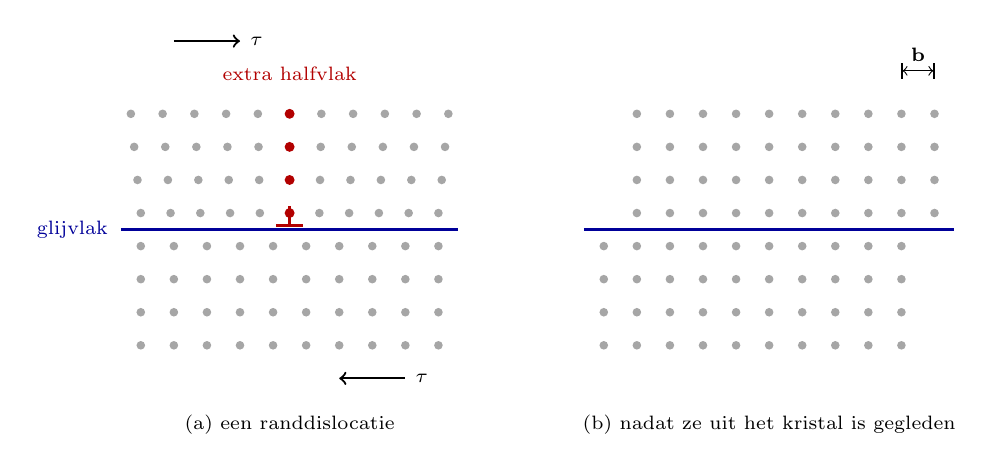
\begin{tikzpicture}[font=\scriptsize, x=0.42cm, y=0.42cm]
% (a) lower half: 10 columns; upper half: 11 columns squeezed over the same width
\foreach \j in {0,...,3} {\foreach \i in {0,...,9} {\fill[gray!70] (\i,\j) circle (0.13);}}
\foreach \j/\s in {4/0.9, 5/0.92, 6/0.94, 7/0.96} {\foreach \i in {0,...,10} {
  \pgfmathsetmacro{\x}{(\i-5)*\s + 4.5}
  \ifnum\i=5 \fill[red!70!black] (\x,\j) circle (0.15); \else \fill[gray!70] (\x,\j) circle (0.13); \fi}}
\draw[thick, blue!60!black] (-0.6,3.5) -- (9.6,3.5);
\node[anchor=east, blue!60!black] at (-0.7,3.5) {glijvlak};
\draw[red!70!black, very thick] (4.1,3.62) -- (4.9,3.62) (4.5,3.62) -- (4.5,4.2);
\node[red!70!black] at (4.5,8.2) {extra halfvlak};
\draw[->, thick] (1.0,9.2) -- (3.0,9.2) node[right] {$\tau$};
\draw[<-, thick] (6.0,-1.0) -- (8.0,-1.0) node[right] {$\tau$};
% (b) after glide: the upper half shifted by one spacing
\begin{scope}[shift={(14,0)}]
\foreach \j in {0,...,3} {\foreach \i in {0,...,9} {\fill[gray!70] (\i,\j) circle (0.13);}}
\foreach \j in {4,...,7} {\foreach \i in {1,...,10} {\fill[gray!70] (\i,\j) circle (0.13);}}
\draw[thick, blue!60!black] (-0.6,3.5) -- (10.6,3.5);
\draw[|<->|] (9,8.3) -- (10,8.3) node[midway, above] {$\mathbf b$};
\end{scope}
\node[anchor=north] at (4.5,-1.8) {(a) een randdislocatie};
\node[anchor=north] at (19,-1.8) {(b) nadat ze uit het kristal is gegleden};
\end{tikzpicture}

\par\smallskip{\small (a) Een randdislocatie: een extra halfvlak van atomen (rood)
eindigt op het glijvlak en vervormt het rooster rond zijn rand (het symbool
$\perp$). Onder de schuifspanning $\tau$ glijdt zij langs het glijvlak door
één rij bindingen tegelijk te breken en opnieuw te vormen. (b) Wanneer zij het
kristal heeft doorkruist, is de bovenste helft met één Burgersvector $\mathbf b$ verschoven, en het
rooster is weer perfect.}\label{fig:b3:deformation-mechanisms:dislocation}
\end{omfigure}

Het rooster verzet zich tegen de glijding van een \omterm{def:b3:deformation-mechanisms:dislocation}{dislocatie} met een kleine spanning, de
Peierls-spanning, die afhangt van de sterkte en de richting van de bindingen:
daarom zijn sommige glijsystemen van een mineraal gemakkelijk en andere moeilijk. Naarmate
een kristal vervormt, vermenigvuldigen \omterm{def:b3:deformation-mechanisms:dislocation}{dislocaties} zich en raken ze verstrengeld; ze blokkeren elkaar, en
het kristal verhardt, tenzij ze obstakels kunnen omklimmen of elkaar kunnen opheffen, wat
diffusie vergt, dus warmte.

\section{Kruipmechanismen}

\begin{definition}[Kruipmechanismen]\label{def:b3:deformation-mechanisms:creep}
Bij \emph{dislocatiekruip}\index{dislocatiekruip} vervormen kristallen door de
glijding van \omterm{def:b3:deformation-mechanisms:dislocation}{dislocaties}, waarbij klimmen hen van obstakels losmaakt. Bij
\emph{diffusiekruip}\index{diffusiekruip} veranderen ze van vorm door de
diffusie van atomen, door het rooster (Nabarro--Herringkruip) of langs de
korrelgrenzen (Coblekruip), van de vlakken onder de hoogste normaalspanning
naar die onder de laagste. Bij \emph{korrelgrensglijding}\index{korrelgrensglijding}
glijden korrels langs elkaar langs hun grenzen, waarbij de openingen
gesloten worden door diffusie of dislocatiekruip. Bij \emph{drukoplossing
}\index{drukoplossing} lost het materiaal op in een vloeistoffilm op de
vlakken onder hoge spanning en wordt afgezet waar de spanning laag is, of
wordt weggevoerd.
\end{definition}

\begin{proposition}[Korrelgrootteafhankelijkheid van diffusiekruip]\label{prop:b3:deformation-mechanisms:grain-size}
Bij lage spanning $\sigma$ kruipt een gesteente met korrelgrootte $d$ door diffusie met de snelheid
\[
  \dot\varepsilon \approx B_L\frac{D_L\Omega}{k_BT}\frac{\sigma}{d^2}
  \quad\text{(door het rooster)},\qquad
  \dot\varepsilon \approx B_B\frac{\delta D_B\Omega}{k_BT}\frac{\sigma}{d^3}
  \quad\text{(langs de grenzen)},
\]
waarin $D_L$ en $D_B$ de diffusiecoëfficiënten zijn in het rooster en in de
grenzen, $\delta$ de breedte van een grens, $\Omega$ het volume van een atoom,
$k_B$ de constante van Boltzmann en $B_L$, $B_B$ getallen van de orde tien die afhangen van
de vorm van de korrels.
\end{proposition}

\begin{proof}
Een normaalspanning $\sigma$ op een vlak verandert het werk dat nodig is om daar een vacature te vormen
met $\sigma\Omega$, zodat de concentratie $C$ van vacatures verschilt tussen vlakken
onder trek en onder druk met $\Delta C \approx C\sigma\Omega/
(k_BT)$ wanneer $\sigma\Omega \ll k_BT$. Over een afstand van de orde $d$ is de
diffusieve flux van vacatures, en dus van atomen in de tegengestelde richting, van de orde $D\Delta
C/d$ per oppervlakte-eenheid. Door het rooster doorkruist de flux een oppervlak van de orde
$d^2$, langs de grenzen een oppervlak van de orde $\delta d$. Het verplaatste volume per
tijdseenheid, gedeeld door het volume van de korrel $d^3$, is de reksnelheid: van de orde
$(D_L\sigma\Omega/k_BT)\,d^2/(d\cdot d^3) = D_L\sigma\Omega/(k_BTd^2)$ in het
rooster, en $(D_B\sigma\Omega/k_BT)\,\delta d/(d\cdot d^3) = \delta D_B
\sigma\Omega/(k_BTd^3)$ in de grenzen. Het product $C\,D$ is de
zelfdiffusiecoëfficiënt, in de opgave $D$ genoemd.
\end{proof}

\omterm{def:b3:deformation-mechanisms:creep}{Diffusiekruip} is lineair in de spanning, een echte viskeuze stroming, en ze verloopt snel in
fijnkorrelig gesteente: halveren van de korrelgrootte maakt Coble-kruip acht keer zo snel
(figuur hieronder). \omterm{def:b3:deformation-mechanisms:creep}{Dislocatiekruip} hangt niet af van de korrelgrootte, maar neemt toe
met een hoge macht van de spanning.

\begin{omfigure}
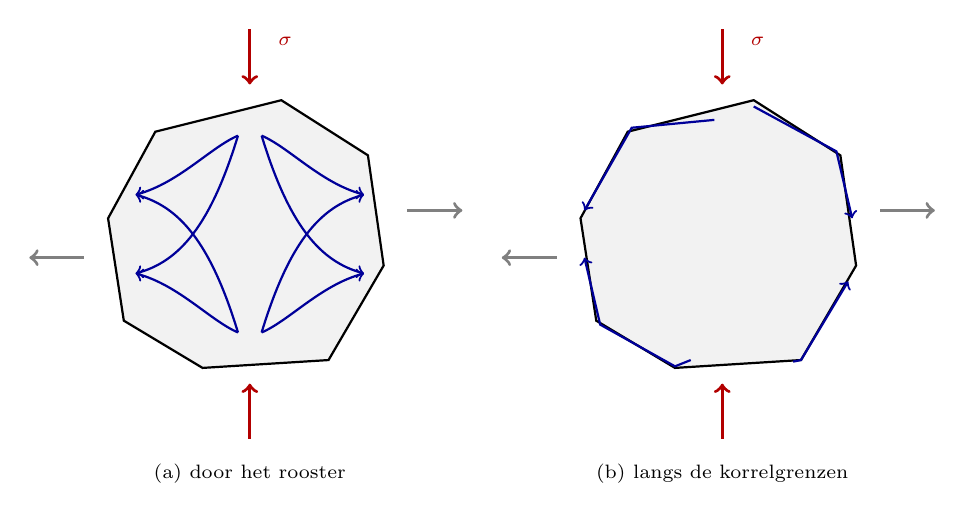
\begin{tikzpicture}[font=\scriptsize, x=1cm, y=1cm]
\foreach \cx/\lab in {0/{(a) door het rooster}, 6/{(b) langs de korrelgrenzen}} {
  \begin{scope}[shift={(\cx,0)}]
  \draw[thick, fill=gray!10] (-1.6,-1.1) -- (-0.6,-1.7) -- (1.0,-1.6) -- (1.7,-0.4) -- (1.5,1.0) -- (0.4,1.7) -- (-1.2,1.3) -- (-1.8,0.2) -- cycle;
  \draw[->, very thick, red!70!black] (0,2.6) -- (0,1.9);
  \draw[->, very thick, red!70!black] (0,-2.6) -- (0,-1.9);
  \node[red!70!black] at (0.45,2.45) {$\sigma$};
  \draw[<-, very thick, gray] (2.7,0.3) -- (2.0,0.3);
  \draw[<-, very thick, gray] (-2.8,-0.3) -- (-2.1,-0.3);
  \node[anchor=north] at (0,-2.8) {\lab};
  \end{scope}
}
\foreach \sx in {1,-1} {\foreach \y in {-0.5,0.5} {
  \draw[->, blue!60!black, thick] (0.15*\sx,1.25) .. controls (0.5*\sx,\y+0.6) and (0.9*\sx,\y+0.15) .. (1.45*\sx,\y);
  \draw[->, blue!60!black, thick] (0.15*\sx,-1.25) .. controls (0.5*\sx,\y-0.6) and (0.9*\sx,\y-0.15) .. (1.45*\sx,\y);
}}
\draw[->, blue!60!black, thick] (6.4,1.62) -- (7.45,1.05) -- (7.65,0.2);
\draw[->, blue!60!black, thick] (5.9,1.45) -- (4.85,1.35) -- (4.25,0.3);
\draw[->, blue!60!black, thick] (6.9,-1.62) -- (7.0,-1.6) -- (7.6,-0.6);
\draw[->, blue!60!black, thick] (5.6,-1.6) -- (5.4,-1.68) -- (4.45,-1.15) -- (4.25,-0.3);
\end{tikzpicture}

\par\smallskip{\small \omterm{def:b3:deformation-mechanisms:creep}{Diffusiekruip} van een korrel die verkort is langs $\sigma$. Atomen
verlaten de vlakken onder de hoogste compressie en worden toegevoegd aan de vlakken onder
de laagste (blauw), zodat de korrel platter wordt en langer (grijze pijlen): (a)
door het binnenste van de korrel, Nabarro--Herring-kruip; (b) langs de grenzen,
Coble-kruip.}\label{fig:b3:deformation-mechanisms:diffusion}
\end{omfigure}

Vervormde kristallen herstellen zich ook terwijl ze vervormen.

\begin{definition}[Herstel, subkorrel, dynamische herkristallisatie]\label{def:b3:deformation-mechanisms:recrystallisation}
\emph{Herstel}\index{herstel (kristalplasticiteit)} is het herschikken van
\omterm{def:b3:deformation-mechanisms:dislocation}{dislocaties}, door klimmen en kruisglijden, tot rangschikkingen met lagere energie, en hun
annihilatie. \omterm{def:b3:deformation-mechanisms:dislocation}{Dislocaties} die in wanden zijn gerangschikt, verdelen een korrel in
\emph{subkorrels}\index{subkorrel}, delen van de korrel waarvan de roosters
een paar graden ten opzichte van elkaar zijn gekanteld. \emph{Dynamische
herkristallisatie}\index{dynamische herkristallisatie} is het vervangen, tijdens
de vervorming, van vervormde korrels door nieuwe korrels met minder \omterm{def:b3:deformation-mechanisms:dislocation}{dislocaties}, hetzij
door de rotatie van subkorrels totdat ze korrels worden, dan wel door de migratie van
korrelgrenzen de sterker vervormde buren in.
\end{definition}

\begin{definition}[Kristallografische voorkeursoriëntatie]\label{def:b3:deformation-mechanisms:cpo}
Een gesteente heeft een \emph{kristallografische voorkeursoriëntatie}\index{kristallografische voorkeursoriëntatie}
(CPO) wanneer de roosters van zijn korrels niet willekeurig georiënteerd zijn
maar zich groeperen rond richtingen die door de vervorming zijn bepaald; \omterm{def:b3:deformation-mechanisms:creep}{dislocatiekruip}
brengt die tot stand door de glijsystemen van elke korrel naar de stroming te roteren.
\end{definition}

Een gesteente met een CPO erft de anisotropie van zijn kristallen: zijn seismische snelheden
hangen bijvoorbeeld af van de richting, waardoor de seismologie de structuur van
de diepe mantel kan waarnemen. \omterm{def:b3:deformation-mechanisms:creep}{Diffusiekruip} en \omterm{def:b3:deformation-mechanisms:creep}{korrelgrensglijding}, die korrels
vrij laten roteren, bouwen er geen op.

\section{Stromingswetten}

\begin{definition}[Stromingswet, spanningsexponent, homologe temperatuur]\label{def:b3:deformation-mechanisms:flow-law}
Een \emph{stromingswet}\index{stromingswet} geeft de reksnelheid van een gesteente dat via één mechanisme
vervormt als functie van de differentiële spanning $\sigma$, de korrelgrootte
$d$, de temperatuur $T$ en de druk $P$:
\[
  \dot\varepsilon = A\,\sigma^nd^{-m}\exp\Bigl(-\frac{E + PV}{RT}\Bigr),
\]
met $A$, $n$, $m$, de activeringsenergie $E$ en het activeringsvolume $V$
in het laboratorium gemeten. De \emph{spanningsexponent}\index{spanningsexponent}
is $n$, de korrelgroottexponent $m$. De \emph{homologe
temperatuur}\index{homologe temperatuur} van een mineraal is $T/T_m$, zijn
absolute temperatuur gedeeld door zijn absolute smelttemperatuur.
\end{definition}

In de hier gebruikte wetten heeft \omterm{def:b3:deformation-mechanisms:creep}{dislocatiekruip} $n$ van 3.5 of 4 en $m = 0$;
\omterm{def:b3:deformation-mechanisms:creep}{diffusiekruip} heeft $n = 1$ en $m = 2$ of 3 (\cref{prop:b3:deformation-mechanisms:grain-size}).
Kruip neemt toe naarmate de \omterm{def:b3:deformation-mechanisms:flow-law}{homologe temperatuur} 1 nadert. Forsteriet smelt bij \qty{1890}{\celsius}, dus de mantel bij \qty{1300}{\celsius}
staat op $T/T_m = 0.73$; ijs bij \qty{-10}{\celsius} op 0.96, waarom
gletsjers stromen. De olivijnwaarden die hier worden gebruikt, zijn die van een veelgebruikte
laboratoriumcompilatie: droge olivijn in \omterm{def:b3:deformation-mechanisms:creep}{dislocatiekruip}, $A =
\num{1.1e5}$, $n = 3.5$, $E = \qty{530}{kJ.mol^{-1}}$, $V =
\qty{14}{cm^3.mol^{-1}}$; in \omterm{def:b3:deformation-mechanisms:creep}{diffusiekruip}, $A = 10^{9.2}$, $n = 1$, $m = 3$,
$E = \qty{375}{kJ.mol^{-1}}$, $V = \qty{5}{cm^3.mol^{-1}}$ (spanning in megapascal,
korrelgrootte in micrometer, tijd in seconden); nat kwartsiet staat in
Boek~3. Water verzwakt olivijn: bij een waterfugaciteit van ongeveer
\qty{300}{MPa}, olivijnaggregaten kruipen vijf tot zes keer sneller dan droge
in \omterm{def:b3:deformation-mechanisms:creep}{dislocatiekruip}, vijf keer sneller in \omterm{def:b3:deformation-mechanisms:creep}{diffusiekruip}.
% ledger: bowen14:mgo-sio2, azuma17:olivine, lopez:flow-laws, codata:R, mk00:diffusion, mk00:dislocation

\begin{proposition}[Effectieve viscositeit]\label{prop:b3:deformation-mechanisms:viscosity}
Een gesteente dat een \omterm{def:b3:deformation-mechanisms:flow-law}{stromingswet} $\dot\varepsilon = A'\sigma^n$ volgt bij gegeven $T$, $P$ en
$d$ heeft de effectieve viscositeit
\[
  \eta_{\mathrm{eff}} = \frac{\sigma}{2\dot\varepsilon}
  = \tfrac12A'^{-1/n}\,\dot\varepsilon^{(1-n)/n}:
\]
voor $n > 1$ daalt zij naarmate het gesteente sneller vervormt.
\end{proposition}

\begin{proof}
Voor een Newtonse vloeistof geldt $\sigma = 2\eta\dot\varepsilon$ in eenassige stroming, volgens de
definitie van viscositeit; $\eta_{\mathrm{eff}}$ is de viscositeit van de Newtonse
vloeistof die onder dezelfde spanning even snel zou stromen. Als men
$\sigma = (\dot\varepsilon/A')^{1/n}$ invult, volgt de tweede vorm.
\end{proof}

Nat kwartsiet dat bij \qty{400}{\celsius} met \qty{e-14}{s^{-1}} vloeit, vergt
\qty{65}{MPa} en heeft een effectieve viscositeit van \qty{3.3e21}{Pa.s}; bij
\qty{500}{\celsius} is dat \qty{18}{MPa} en \qty{9e20}{Pa.s}: honderd graden
extra deelt de sterkte door meer dan drie (zie figuur hieronder). Droge olivijn bij
\qty{1100}{\celsius} en \qty{1}{GPa} vergt slechts \qty{3}{MPa}.
De sterkte-enveloppen van Boek~3 zijn opgebouwd uit precies deze wetten.

\begin{omfigure}
\begin{tikzpicture}
\begin{groupplot}[group style={group size=2 by 1, horizontal sep=1.6cm},
  omrecord, width=0.47\linewidth, height=0.47\linewidth, xmode=log,
  xmin=1, xmax=1000, ymin=-20, ymax=-6, xlabel={differentiële spanning (MPa)},
  legend style={font=\scriptsize, at={(0.97,0.03)}, anchor=south east, legend columns=1}]
\nextgroupplot[ylabel={$\log_{10}\dot\varepsilon$ (\unit{s^{-1}})}, title={(a) nat kwartsiet},
  title style={font=\small}]
% computed in figdata/bachelor-3/flow_laws.py; ledger: lopez:flow-laws, azuma17:olivine
\addplot[omDef, thick] table[x=s, y=r600] {figdata/out/bachelor-3-flow_laws-quartz.dat};
\addlegendentry{\qty{600}{\celsius}}
\addplot[red!70!black, thick, densely dashed] table[x=s, y=r500] {figdata/out/bachelor-3-flow_laws-quartz.dat};
\addlegendentry{\qty{500}{\celsius}}
\addplot[black, thick, densely dotted] table[x=s, y=r400] {figdata/out/bachelor-3-flow_laws-quartz.dat};
\addlegendentry{\qty{400}{\celsius}}
\draw[gray] (axis cs:1,-14) -- (axis cs:1000,-14);
\nextgroupplot[title={(b) droge olivijn, \qty{1}{GPa}}, title style={font=\small}]
\addplot[omDef, thick] table[x=s, y=r1300] {figdata/out/bachelor-3-flow_laws-olivine.dat};
\addlegendentry{\qty{1300}{\celsius}}
\addplot[red!70!black, thick, densely dashed] table[x=s, y=r1100] {figdata/out/bachelor-3-flow_laws-olivine.dat};
\addlegendentry{\qty{1100}{\celsius}}
\addplot[black, thick, densely dotted] table[x=s, y=r900] {figdata/out/bachelor-3-flow_laws-olivine.dat};
\addlegendentry{\qty{900}{\celsius}}
\draw[gray] (axis cs:1,-14) -- (axis cs:1000,-14);
\end{groupplot}
\end{tikzpicture}

\par\smallskip{\small Stromingswetten voor \omterm{def:b3:deformation-mechanisms:creep}{dislocatiekruip}: vervormingssnelheid tegen spanning bij
drie temperaturen. De helling op deze assen is de \omterm{def:b3:deformation-mechanisms:flow-law}{spanningsexponent}, 4 voor
kwartsiet en 3.5 voor olivijn; de grijze lijn markeert een geologische vervormingssnelheid,
\qty{e-14}{s^{-1}}. Olivijn heeft temperaturen nodig die ongeveer \qty{600}{\celsius}
hoger liggen dan die van kwarts om even gemakkelijk te stromen.}\label{fig:b3:deformation-mechanisms:flow-laws}
\end{omfigure}

\section{Vervormingsmechanismekaarten}

Meerdere mechanismen werken naast elkaar, en het snelste draagt de vervorming.

\begin{definition}[Vervormingsmechanismekaart]\label{def:b3:deformation-mechanisms:deformation-map}
Een \emph{vervormingsmechanismekaart}\index{vervormingsmechanismekaart} van een
mineraal of gesteente toont, op assen van twee van de variabelen spanning, korrelgrootte en
temperatuur, de velden waarin elk mechanisme het snelst is, met contouren
van de totale vervormingssnelheid.
\end{definition}

\begin{proposition}[Grens tussen mechanismen]\label{prop:b3:deformation-mechanisms:boundary}
Bij gegeven $T$ en $P$ lopen \omterm{def:b3:deformation-mechanisms:creep}{dislocatiekruip} ($A_1$, $n_1$, $E_1$, $V_1$, geen
korrelgrootteafhankelijkheid) en \omterm{def:b3:deformation-mechanisms:creep}{diffusiekruip} ($A_2$, $n_2 = 1$, $m$, $E_2$, $V_2$)
even snel bij de spanning
\[
  \sigma_b = \biggl(\frac{A_2d^{-m}}{A_1}
  \exp\frac{(E_1 - E_2) + P(V_1 - V_2)}{RT}\biggr)^{1/(n_1 - 1)} ,
\]
De grens is dus een rechte lijn met helling $-m/(n_1 - 1)$ op logaritmische
assen van korrelgrootte en spanning; boven die grens wint \omterm{def:b3:deformation-mechanisms:creep}{dislocatiekruip}.
\end{proposition}

\begin{proof}
Stel de twee stromingswetten gelijk en los op naar $\sigma$. Boven $\sigma_b$ is de verhouding van
de twee snelheden, evenredig met $\sigma^{n_1 - 1}$, groter dan 1.
\end{proof}

Voor droge olivijn bij \qty{1100}{\celsius} en \qty{2}{GPa} ligt de grens bij
\qty{5}{MPa} voor een korrelgrootte van \qty{1}{mm} en bij \qty{79}{MPa} voor
\qty{100}{\micro m} (zie figuur hieronder). Fijnkorrelige mantel kruipt door diffusie,
grofkorrelige mantel door \omterm{def:b3:deformation-mechanisms:dislocation}{dislocaties}; laboratorium- en geofysisch bewijs suggereert
dat beide regimes in de bovenmantel voorkomen, waarbij de hete, ondiepe mantel door
\omterm{def:b3:deformation-mechanisms:creep}{dislocatiekruip} stroomt en de koudere of diepere door \omterm{def:b3:deformation-mechanisms:creep}{diffusiekruip}, en dat waar
de spanning stijgt en de korrels krimpen, de mantel nabij de grens verzwakt
en de vervorming lokaliseert.
% ledger: azuma17:olivine, karato93:transitions

\begin{omfigure}
\begin{tikzpicture}
\begin{axis}[omrecord, xmode=log, ymode=log, width=0.78\linewidth, height=0.58\linewidth,
  xmin=10, xmax=1e4, ymin=0.01, ymax=1000, xlabel={korrelgrootte (\unit{\micro m})},
  ylabel={differentiële spanning (MPa)}, clip=true]
% computed in figdata/bachelor-3/flow_laws.py; ledger: azuma17:olivine
\addplot[black, very thick] table[x=d, y=s] {figdata/out/bachelor-3-flow_laws-mapbound.dat};
\foreach \c in {16,14,12,10} {
  \addplot[omDef, thick] table[x=d, y=s\c] {figdata/out/bachelor-3-flow_laws-mapcont.dat};
}
\node[font=\scriptsize, fill=white, inner sep=1pt] at (axis cs:7000,1.15) {$10^{-16}$};
\node[font=\scriptsize, fill=white, inner sep=1pt] at (axis cs:7000,4.2) {$10^{-14}$};
\node[font=\scriptsize, fill=white, inner sep=1pt] at (axis cs:7000,15.7) {$10^{-12}$};
\node[font=\scriptsize, fill=white, inner sep=1pt] at (axis cs:4200,58) {$10^{-10}\,\unit{s^{-1}}$};
\node[font=\small, anchor=north east] at (axis cs:9000,600) {dislocatiekruip};
\node[font=\small, anchor=south west] at (axis cs:1500,0.013) {diffusiekruip};
\end{axis}
\end{tikzpicture}

\par\smallskip{\small \omterm{def:b3:deformation-mechanisms:deformation-map}{Vervormingsmechanismekaart} van droge olivijn bij
\qty{1100}{\celsius} en \qty{2}{GPa}. De dikke lijn scheidt de velden waar
\omterm{def:b3:deformation-mechanisms:creep}{dislocatiekruip} (boven) en \omterm{def:b3:deformation-mechanisms:creep}{diffusiekruip} (onder) sneller is; de dunne lijnen
zijn contouren van de totale vervormingssnelheid, vlak waar \omterm{def:b3:deformation-mechanisms:creep}{dislocatiekruip}, dat
de korrelgrootte negeert, overheerst.}\label{fig:b3:deformation-mechanisms:map}
\end{omfigure}

De korrelgrootte die \omterm{def:b3:deformation-mechanisms:recrystallisation}{dynamische herkristallisatie} voortbrengt, hangt af van de spanning,
en dit maakt de korrels tot een spanningsmeter.

\begin{definition}[Paleopiëzometer]\label{def:b3:deformation-mechanisms:piezometer}
Een \emph{paleopiëzometer}\index{paleopiëzometer} is een kenmerk van een vervormd
gesteente waarvan de grootte of dichtheid wordt bepaald door de differentiële spanning waaronder
het is gevormd, in het laboratorium gekalibreerd, waaruit de spanning van een
vroegere vervorming kan worden afgelezen.
\end{definition}

Voor kwarts leverden experimenten bij \qty{1.5}{GPa} en 800 tot \qty{1100}{\celsius}, bij
vloeispanningen van 34 tot \qty{268}{MPa}, herkristalliseerde korrels van 46 tot
\qty{3.2}{\micro m}, benaderd door
\[
  D = 10^{3.56}\,\sigma^{-1.26}\qquad(D\text{ in \unit{\micro m}},\ \sigma\text{ in MPa}),
\]
zonder meetbaar effect van de temperatuur. Een kwartsmyloniet met
herkristalliseerde korrels van \qty{20}{\micro m} doorsnede is vervormd onder ongeveer
\qty{62}{MPa}.
% ledger: st03:piezometer

\section{Schuifzones}

\begin{definition}[Schuifzone, rekverzachting]\label{def:b3:deformation-mechanisms:shear-zone}
Een \emph{schuifzone}\index{schuifzone} is een plaatvormige zone, tussen wanden die
weinig vervormd zijn, waarin de rek is geconcentreerd en die nagenoeg een
eenvoudige schuif evenwijdig aan de zone is. Een gesteente ondergaat \emph{rekverzachting}\index{rekverzachting}
wanneer zijn sterkte afneemt naarmate het vervormt.
\end{definition}

\omterm{def:b3:deformation-mechanisms:shear-zone}{Rekverzachting} zorgt ervoor dat een \omterm{def:b3:deformation-mechanisms:shear-zone}{schuifzone} smal blijft: zodra een band zwakker is
dan zijn wanden, blijft de vervorming erin. Korrelgroottereductie door \omterm{def:b3:deformation-mechanisms:recrystallisation}{dynamische
herkristallisatie}, die het gesteente in \omterm{def:b3:deformation-mechanisms:creep}{diffusiekruip} kan doen overgaan, de groei van een
\omterm{def:b3:deformation-mechanisms:cpo}{kristallografische voorkeursoriëntatie} die gemakkelijke glijsystemen uitlijnt, het binnendringen van water en reacties die
zwakke mineralen, zoals micas, vormen, verzachten allemaal het gesteente. De mylonieten uit Boek~3 zijn hiervan het product.
In een \omterm{def:b3:deformation-mechanisms:shear-zone}{schuifzone} van eenvoudige schuif wordt een merker die de zone loodrecht kruist
in de zone afgebogen: bevindt hij zich binnen de zone, dan maakt hij de hoek
$\psi$ met zijn oorspronkelijke richting, en de schuifrek is $\gamma
= \tan\psi$, en de verplaatsing over een zone met breedte $w$ is $\gamma w$.

\begin{definition}[Kinematische indicatoren]\label{def:b3:deformation-mechanisms:kinematic}
Een \emph{kinematische indicator}\index{kinematische indicator} is een structuur waarvan de
asymmetrie de \emph{schuifzin}\index{schuifzin} vastlegt, de richting waarin de ene wand van een
\omterm{def:b3:deformation-mechanisms:shear-zone}{schuifzone} ten opzichte van de andere is bewogen, af te lezen in het vlak dat de rekkingslineatie
bevat en loodrecht op de foliatie staat.
Een \emph{S--C-maaksel}\index{S--C-maaksel} is een paar foliaties: S, de
foliatie van afgeplatte korrels, schuin op de zone en naar de
rekrichting gedraaid, en C, schuifbanden evenwijdig aan de zone. Een
\emph{porfiroklastsysteem}\index{porfiroklastsysteem} is een sterke korrel met
staarten van herkristalliseerd materiaal: bij een $\sigma$-type lopen de staarten van de ene
kant van de middellijn van de kloast naar de andere zonder die te kruisen, bij een $\delta$-type,
meegesleept door de rotatie van de kloast, kruisen ze die. Een
\emph{micavis}\index{micavis} is een ruitvormige miccorrel die schuin op
het schuifvlak staat, met dunne staarten, die trapsgewijs lopen zoals die van een $\sigma$-type kloast.
\end{definition}

\begin{omfigure}
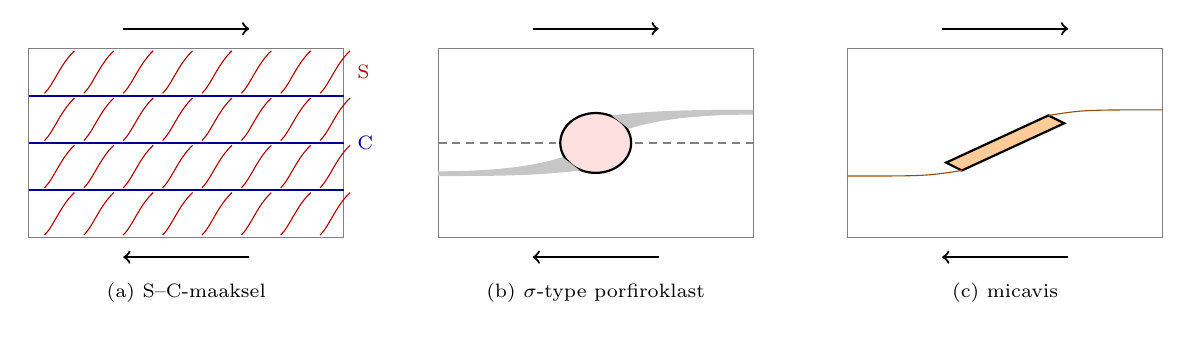
\begin{tikzpicture}[font=\scriptsize, x=1cm, y=1cm]
% (a) S-C fabric, dextral
\begin{scope}
\draw[gray] (0,0) rectangle (4,2.4);
\foreach \y in {0.6,1.2,1.8} {\draw[blue!60!black, thick] (0,\y) -- (4,\y);}
\foreach \y in {0,0.6,1.2,1.8} {\foreach \x in {0.2,0.7,...,3.8} {
  \draw[red!70!black] (\x,\y+0.03) .. controls (\x+0.12,\y+0.15) and (\x+0.2,\y+0.4) .. (\x+0.38,\y+0.57);}}
\draw[->, thick] (1.2,2.65) -- (2.8,2.65);
\draw[<-, thick] (1.2,-0.25) -- (2.8,-0.25);
\node[anchor=north] at (2,-0.45) {(a) S--C-maaksel};
\node[blue!60!black, anchor=west] at (4.05,1.2) {C};
\node[red!70!black, anchor=west] at (4.05,2.1) {S};
\end{scope}
% (b) sigma clast
\begin{scope}[shift={(5.2,0)}]
\draw[gray] (0,0) rectangle (4,2.4);
\fill[red!12] (2.0,1.2) ellipse (0.45 and 0.38);
\draw[thick] (2.0,1.2) ellipse (0.45 and 0.38);
\fill[gray!45] (2.2,1.55) .. controls (2.8,1.62) and (3.3,1.62) .. (4.0,1.62) -- (4.0,1.56) .. controls (3.3,1.56) and (2.8,1.5) .. (2.42,1.38) -- cycle;
\fill[gray!45] (1.8,0.85) .. controls (1.2,0.78) and (0.7,0.78) .. (0,0.78) -- (0,0.84) .. controls (0.7,0.84) and (1.2,0.9) .. (1.58,1.02) -- cycle;
\draw[gray, densely dashed] (0,1.2) -- (1.5,1.2) (2.5,1.2) -- (4,1.2);
\draw[->, thick] (1.2,2.65) -- (2.8,2.65);
\draw[<-, thick] (1.2,-0.25) -- (2.8,-0.25);
\node[anchor=north] at (2,-0.45) {(b) $\sigma$-type porfiroklast};
\end{scope}
% (c) mica fish
\begin{scope}[shift={(10.4,0)}]
\draw[gray] (0,0) rectangle (4,2.4);
\fill[orange!40] (1.25,0.95) -- (2.55,1.55) -- (2.75,1.45) -- (1.45,0.85) -- cycle;
\draw[thick] (1.25,0.95) -- (2.55,1.55) -- (2.75,1.45) -- (1.45,0.85) -- cycle;
\draw[orange!60!black] (2.55,1.55) .. controls (3.0,1.62) .. (4.0,1.62);
\draw[orange!60!black] (1.45,0.85) .. controls (1.0,0.78) .. (0,0.78);
\draw[->, thick] (1.2,2.65) -- (2.8,2.65);
\draw[<-, thick] (1.2,-0.25) -- (2.8,-0.25);
\node[anchor=north] at (2,-0.45) {(c) micavis};
\end{scope}
\end{tikzpicture}

\par\smallskip{\small Drie \omterm{def:b3:deformation-mechanisms:kinematic}{kinematische indicatoren} van dezelfde rechtse schuif
(bovenkant naar rechts, pijlen), gezien in het vlak van de lineatie, loodrecht op de
foliatie. (a) De S-foliatie (rood) buigt om in de C-schuifbanden (blauw),
en helt in de richting van de rekking. (b) De staarten van een $\sigma$-type kloast
verlaten de bovenzijde naar rechts en de onderzijde naar links, en lopen trapsgewijs op in
de schuifrichting zonder de middellijn (gestippeld) te kruisen. (c) Een
\omterm{def:b3:deformation-mechanisms:kinematic}{micavis} helt als S, en zijn staarten lopen trapsgewijs zoals die van een $\sigma$-type kloast. Niet
op schaal.}\label{fig:b3:deformation-mechanisms:kinematic}
\end{omfigure}

Samen gelezen geven een paar indicatoren die overeenstemmen de \omterm{def:b3:deformation-mechanisms:kinematic}{schuifzin} met
vertrouwen; een enkele kan misleiden, want er bestaan teruggedraaide kloasten en
asymmetrische plooien van andere oorsprong. De foto in het kader hieronder toont
porfiroklasten in een myloniet.

\begin{inthelab}[Gesteente samendrukken bij manteltoestanden]
\begin{minipage}[t]{0.55\linewidth}\vspace{0pt}
In een gasmedium-vervormingsapparaat wordt een cilinder van gesteente of van heetgeperst
olivijnpoeder, een of twee centimeter lang, ingesloten in een dunne metalen mantel en
met zijn zuigers in een oven geplaatst, in een stalen vat gevuld met een
samengeperst inert gas dat de insluitdruk instelt, enkele honderden megapascal.
Een actuator drijft de zuiger aan met een constante snelheid, of onder een
constante belasting, terwijl een interne krachtcel de spanning meet op het monster
zelf, vrij van de wrijving van de afdichtingen. Olivijn wordt op deze manier
vervormd bij temperaturen nabij \qty{1200}{\celsius}; aan het eind van een run
wordt het monster snel afgekoeld, gesneden, gepolijst en onder de microscoop en
de elektronenmicroscoop bekeken, waar de korrelgrootte, \omterm{def:b3:deformation-mechanisms:recrystallisation}{subkorrels} en \omterm{def:b3:deformation-mechanisms:dislocation}{dislocaties} worden gemeten.
\end{minipage}\hfill
\begin{minipage}[t]{0.42\linewidth}\vspace{0pt}
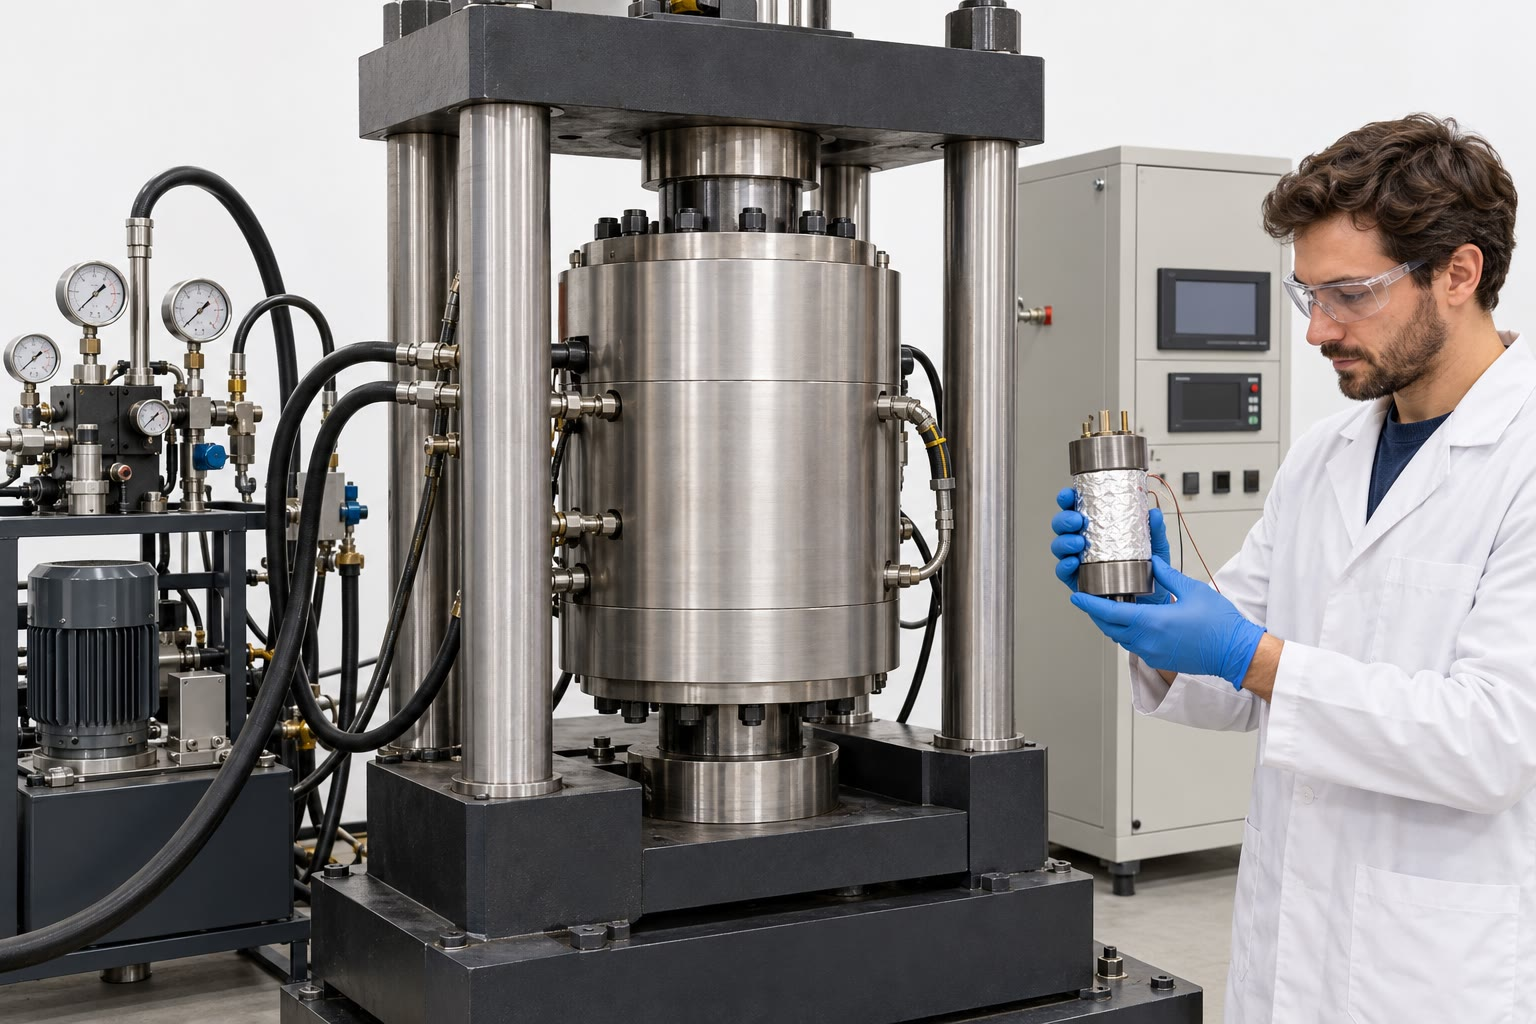
\includegraphics[width=\linewidth]{images/book5/ai/b3-deformation-press.jpg}

{\scriptsize Een gesteentevervormingspers met een gemanteld monsterassemblage.
Door AI gegenereerde illustratie.}

\smallskip
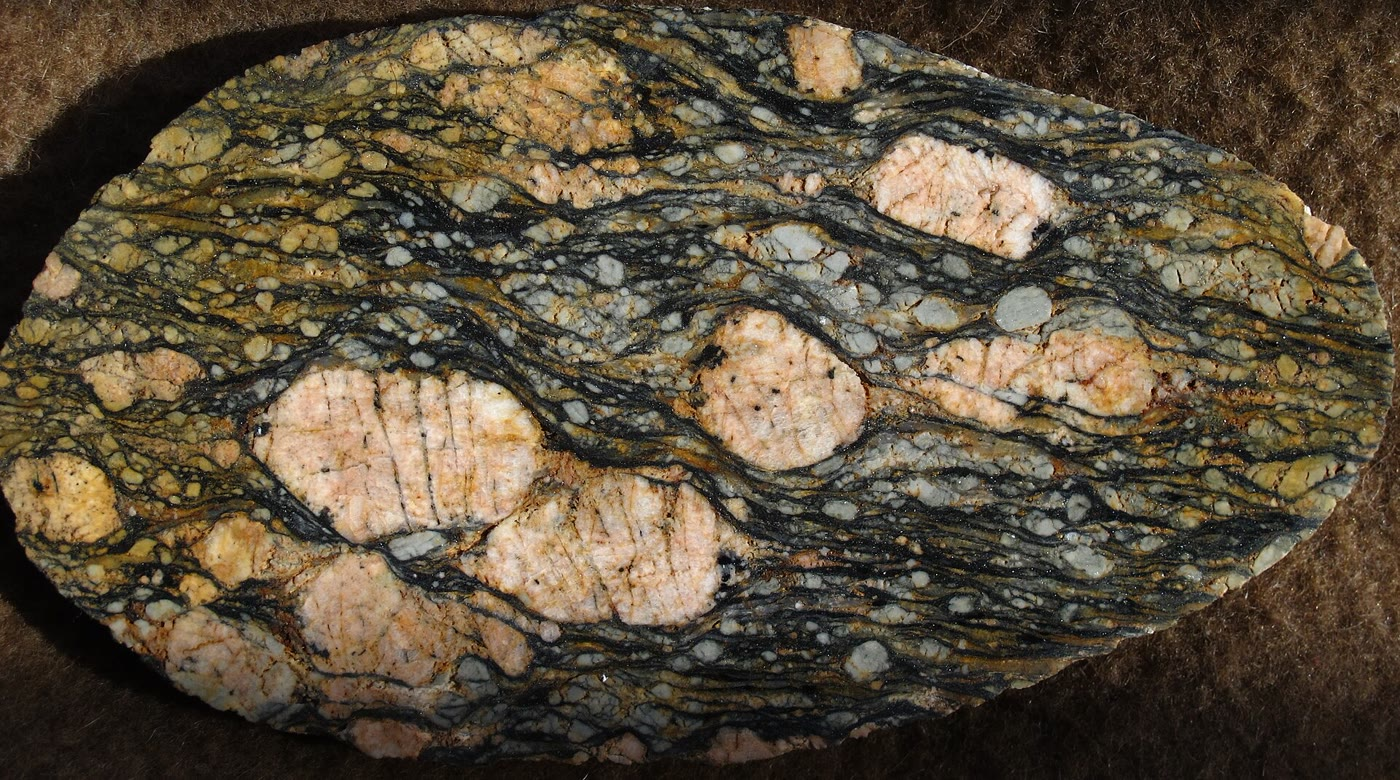
\includegraphics[width=\linewidth]{images/book5/b3-augen-mylonite.jpg}

{\scriptsize Een gezaagde augenmyloniet uit Noorwegen: grote veldspaatporfiroklasten
in een fijne matrix van gerekristalliseerd kwarts, veldspaat en micas. Foto
Mikenorton, CC BY-SA 4.0.}
\end{minipage}
\end{inthelab}
% ledger: mk00:diffusion, photo:b3-augen-mylonite

\section{Oefeningen}

\begin{exercise}[$\star$]\label{exo:b3:deformation-mechanisms:1}
Forsteriet smelt bij \qty{1890}{\celsius} en ijs bij \qty{0}{\celsius}. Bereken
de \omterm{def:b3:deformation-mechanisms:flow-law}{homologe temperatuur} van forsteriet bij \qty{1300}{\celsius} en van ijs bij
\qty{-10}{\celsius}. Welke kruipt makkelijker?
\end{exercise}

\begin{exercise}[$\star$]\label{exo:b3:deformation-mechanisms:2}
Een gang die een \omterm{def:b3:deformation-mechanisms:shear-zone}{schuifzone} loodrecht kruist, wordt binnen de zone
over \ang{70} afgebogen, en een andere over \ang{80}. Bereken de schuifrekken.
Waarom zijn grote rekken op deze manier moeilijk te meten?
\end{exercise}

\begin{exercise}[$\star$]\label{exo:b3:deformation-mechanisms:3}
Welke spanning past bij een gerekristalliseerde korrelgrootte van
\qty{10}{\micro m}, volgens de kwartspiëzometer?
\end{exercise}

\begin{exercise}[$\star$]\label{exo:b3:deformation-mechanisms:4}
Met de vloeiwet van nat kwartsiet ($A = \num{1.1e-4}$, $n = 4$, $E =
\qty{223}{kJ.mol^{-1}}$), $R = \qty{8.314}{J.mol^{-1}.K^{-1}}$), bereken de
reksnelheid bij \qty{500}{\celsius} onder \qty{20}{MPa}.
\end{exercise}

\begin{exercise}[$\star\star$]\label{exo:b3:deformation-mechanisms:5}
Bereken de effectieve viscositeit van nat kwartsiet dat stroomt bij \qty{e-14}{s^{-1}}
bij \qty{400}{\celsius} (\qty{65.4}{MPa}) en bij \qty{500}{\celsius}
(\qty{18.0}{MPa}). Vergelijk met de manteltviscositeiten
in \cref{ch:b3:mantle-convection}.
\end{exercise}

\begin{exercise}[$\star\star$]\label{exo:b3:deformation-mechanisms:6}
Twee experimenten bij dezelfde temperatuur geven \qty{e-5}{s^{-1}} onder
\qty{100}{MPa} en \qty{1.6e-4}{s^{-1}} onder \qty{200}{MPa}. Bereken de
\omterm{def:b3:deformation-mechanisms:flow-law}{spanningsexponent} en noem het waarschijnlijke mechanisme.
\end{exercise}

\begin{exercise}[$\star\star$]\label{exo:b3:deformation-mechanisms:7}
Bij dezelfde spanning kruipt een monster tien keer zo snel bij \qty{1100}{K} als
bij \qty{1000}{K}. Bereken de activeringsenergie.
\end{exercise}

\begin{exercise}[$\star\star$]\label{exo:b3:deformation-mechanisms:8}
Met welke factor verandert de reksnelheid van \omterm{def:b3:deformation-mechanisms:creep}{diffusiekruip} wanneer de
korrelgrootte tien keer kleiner wordt, voor Nabarro--Herring- en voor
Coble-kruip? Waarom is Coble-kruip gevoeliger?
\end{exercise}

\begin{exercise}[$\star\star$]\label{exo:b3:deformation-mechanisms:9}
Voor droge olivijn bij \qty{1100}{\celsius} en \qty{2}{GPa} geven de twee vloeiwetten
$\dot\varepsilon_{\mathrm{dis}} = \num{6.54e-17}\,\sigma^{3.5}$ en
$\dot\varepsilon_{\mathrm{dif}} = \num{3.59e-6}\,\sigma d^{-3}$ (eenheden van de
tekst). Bereken de grensspanning voor $d = \qty{1}{mm}$ en $d =
\qty{100}{\micro m}$, en de helling van de grens.
\end{exercise}

\begin{exercise}[$\star\star\star$]\label{exo:b3:deformation-mechanisms:10}
Volg het bewijs van \cref{prop:b3:deformation-mechanisms:grain-size},
verklaar waarom het roosterpad $d^{-2}$ geeft en het grenspad $d^{-3}$, en toon aan
dat grensdiffusie wint onder de korrelgrootte $d^* \approx
(B_B/B_L)\,\delta D_B/D_L$.
\end{exercise}

\begin{exercise}[$\star\star\star$]\label{exo:b3:deformation-mechanisms:11}
Voor een vloeiwet met $n = 3.5$, met welke factor daalt de effectieve
viscositeit wanneer de reksnelheid tien keer zo groot wordt? Waarom begunstigt dit
de lokalisatie van rek in \omterm{def:b3:deformation-mechanisms:shear-zone}{schuifzones}?
\end{exercise}

\begin{exercise}[$\star\star\star$]\label{exo:b3:deformation-mechanisms:12}
In de droge olivijn van oefening 9 rekristalliseert een manteschuifzone onder \qty{10}{MPa}
van \qty{3}{mm} tot \qty{30}{\micro m} grote korrels. Bereken de totale reksnelheid
vóór en na, en de verzachtingsfactor. Welk mechanisme draagt de vervorming
in beide gevallen?
\end{exercise}

\section{Probleem: De Varden-schuifzone}

\begin{problem}[{Weekendprobleem --- de rek, spanning, reksnelheid en ouderdom van een
verzonnen schuifzone}]
\label{pb:b3:deformation-mechanisms:1}
% values: calc/ch07.py; flow_laws.py; st03:piezometer, lopez:flow-laws
Onder de graniet van de Varden Hills, het verzonnen gebied van de reeks, onthullen een
boorgat en een diepe wegsnede (beide verzonnen) een ductiele \omterm{def:b3:deformation-mechanisms:shear-zone}{schuifzone}
van \qty{400}{m} breed, gevormd op ongeveer \qty{15}{km} diepte en bij \qty{450}{\celsius}.
Een dolerietgang die de wanden loodrecht kruist, maakt binnen de zone
een hoek van slechts \ang{6} met de grenzen van de zone. Het kwarts ervan is een myloniet
van gerekristalliseerde korrels van \qty{20}{\micro m} breed (van 15 tot
\qty{25}{\micro m}). Neem de kwartspiëzometer $D = 10^{3.56}\sigma^{-1.26}$,
de vloeiwet van nat kwartsiet ($A = \num{1.1e-4}$, $n = 4$, $E =
\qty{223}{kJ.mol^{-1}}$), $R = \qty{8.314}{J.mol^{-1}.K^{-1}}$, \qty{1}{yr} $=
\qty{3.156e7}{s}$, en, bij eenvoudige schuif, $\dot\gamma = 2\dot\varepsilon$.

\medskip\noindent\textbf{Deel I --- De rek.}
\begin{enumerate}
  \item Bereken de afbuiging $\psi$ van de gang en de schuifrek.
  \item Bereken de verplaatsing van de ene wand ten opzichte van de andere.
  \item Bereken de hoofdrekken van de rekellips en
        de asverhouding ervan.
  \item Bereken de hoek van de lange as met de zone. Wat doet de
        foliatie van de zone naarmate $\gamma$ toeneemt?
  \item Gezien van bovenaf buigt de gang, gevolgd vanaf de zuidelijke wand, naar het
        oosten zodra hij de oost--west-zone binnengaat, en keert dan
        terug naar zijn noordelijke koers bij de noordelijke wand. In welke
        richting bewoog de noordelijke wand, en is de zone dextraal of sinistraal?
  \item In welk vlak moet een slijpplaatje worden gesneden om de \omterm{def:b3:deformation-mechanisms:kinematic}{kinematische
        indicatoren} af te lezen, en hoe moet zijn S-foliatie hellen?
\end{enumerate}

\medskip\noindent\textbf{Deel II --- De spanning.}
\begin{enumerate}[resume]
  \item Bereken de spanning die de korrels van \qty{20}{\micro m} aangeven.
  \item Bereken de spanningen voor 15 en \qty{25}{\micro m}.
  \item Valt de spanning binnen het bereik van de kalibratie?
  \item De piëzometer vertoonde geen effect van temperatuur. Waarom is dat hier
        van belang?
  \item Welke korrelgrootte had een spanning van \qty{100}{MPa} opgeleverd?
\end{enumerate}

\medskip\noindent\textbf{Deel III --- De reksnelheid.}
\begin{enumerate}[resume]
  \item Bereken $E/RT$ bij \qty{450}{\celsius} en de Arrheniusfactor.
  \item Bereken de reksnelheid van het kwarts onder de spanning van vraag 7
        (neem \qty{62}{MPa}).
  \item Bereken de schuifreksnelheid.
  \item Bereken de effectieve viscositeit van de zone en vergelijk die met de
        bovenmantel van \cref{ch:b3:mantle-convection}.
  \item Met welke factoren zou de reksnelheid veranderen bij 400 en
        \qty{500}{\celsius}, bij dezelfde spanning?
  \item Met welke factor als de spanning de \qty{78}{MPa} van de fijnste
        korrels zou zijn?
\end{enumerate}

\medskip\noindent\textbf{Deel IV --- De tijd.}
\begin{enumerate}[resume]
  \item Bereken de tijd die nodig is om de schuifrek van vraag 1 op te bouwen,
        in seconden.
  \item Reken die om naar duizenden jaren.
  \item Bereken de gemiddelde verschuivingssnelheid over de zone, in \unit{mm/yr}.
  \item Vergelijk die met plaatgrenssnelheden van tientallen millimeters per jaar.
        % ledger: morvel:range
  \item Als de zone \qty{20}{mm/yr} had gedragen, welke schuifreksnelheid, spanning
        en gerekristalliseerde korrelgrootte zou hij dan hebben gehad?
  \item Hoe werken de onzekerheden van de korrelgrootte en die van de
        exponent van de piëzometer door op de tijd?
  \item Geef de tijd die de \omterm{def:b3:deformation-mechanisms:shear-zone}{Varden-schuifzone} nodig had om zijn rek op te bouwen, in
        duizenden jaren.
\end{enumerate}
\end{problem}
